\documentclass[a4paper,titlepage]{article}
\usepackage{frontespizio}
\usepackage[italian]{babel}
\usepackage[utf8]{inputenc}
\usepackage{usecases}
\usepackage{listings}
\usepackage{verbatim}
\usepackage{tikz}
\usepackage{pdfpages}
\usepackage{color}
\usetikzlibrary{arrows,shadows} % for pgf-umlsd
\usepackage[underline=true,rounded corners=false]{pgf-umlsd}
\usepackage{enumitem}
\setitemize{noitemsep,topsep=0pt,parsep=0pt,partopsep=0pt}
\usepackage[a4paper, total={6in, 9in}]{geometry}

\lstset {
basicstyle=\small,
escapeinside=\`\`,
breaklines=true
}


\begin{document}
\begin{frontespizio}
\Universita{Verona}
\Dipartimento{Informatica}
\Corso[Laurea]{Informatica}
\Titoletto{Basi di Dati}
\Titolo{Elaborato G33\\Sistema informativo per cartelle cliniche\\di una divisione ospedaliera}

\Candidato[VR359169]{Enrico Giordano}
\Candidato[VR361121]{Cristian Pinna}

\Annoaccademico{2013-2014}
\end{frontespizio}

\tableofcontents

\newpage

\part{Testo dell'elaborato}
\emph{\textbf{\Large{Requisiti}}}

\noindent
\emph{\textbf{\large{Base di dati}}}

\noindent
Si vuole progettare un sistema informativo per gestire le cartelle cliniche di una divisione ospedaliera. Ogni cartella clinica è caratterizzata dall'indicazione del paziente a cui fa riferimento, dalla data di ricovero, dalla data di dimissione, dal motivo del ricovero e dalla prognosi effettuata al termine del ricovero. Ogni cartella clinica è dotata di un codice indentificativo univoco.\par
\noindent
Per ogni paziente sono memorizzati: il codice sanitario univoco (login), una password, il cognome, il nome, la data di nascita, il luogo di nascita, l'indirizzo di residenza (via, civico, cap, città, provincia). Per ogni paziente è possibile memorizzare gli eventuali fattori di rischio presenti (anche più d'uno).\par
\noindent
Nella cartella clinica si tiene traccia di tutto quanto succede al paziente considerato. In particolare, si registrano le terapie somministrate, caratterizzate da: farmaco somministrato, dose, frequenza giornaliera, data di inizio e data di fine della terapia stessa. Vengono registrati, poi, tutti i sintomi dichiarati dal paziente nel corso del ricovero: i sintomi sono caratterizzati dal nome, dall'intensità, dalla data di insorgenza, dalla durata (non specificata per i sintomi in corso).\par
\noindent
Infine vengono registrate le diagnosi effettuate dai medici sui pazienti: ogni diagnosi è caratterizzata dal paziente considerato, dalla data in cui la diagnosi è effettuata, dal medico che l'ha effettuata, dalla codifica univoca ICD10 della patologia individuata (ICD10 è una classificazione internazionale delle patologie adottata in numerosi stati e organizzazioni sanitarie), e dal nome della patologia individuata. Ogni diagnosi è legata ai sintomi che la confermano e ai sintomi contraddittori, che, invece, potrebbero mettere in discussione la diagnosi considerata. Possono esserci più diagnosi su un paziente nella stessa cartella clinica.\par
\noindent
Per ogni medico si registra: il cognome, il nome, l'elenco delle specializzazioni, data di inizio attività, una matricola univoca (login) e una password. Tra i medici si indica anche il primario della divisione.\newline
\newline
\emph{\textbf{\large{Sito web}}}

\noindent
Le informazioni contenute nella base di dati devono essere presentate in un sito web. Tale sito deve essere stutturato in schemi di pagina come di seguito descritto; è possibile estendere la struttura aggiungendo ulteriori schemi di pagina che mostrano ulteriori dettagli:
\noindent
\begin{itemize}[leftmargin=0.75cm, labelsep= 0.5cm]

\item \textbf{HomePage}, dove si riporta:
	\begin{itemize}[leftmargin=1.5cm, labelsep= 0.5cm, label=$\circ$]

	\item La presentazione della divisione ospedaliera
	\item Varie foto della divisione
	\item Il nome e il cognome del primario
	\item Una form che richiede login e password del paziente per l'accesso alle pagine riservate \textbf{(PazientePage)}
	\item Un link statico al personale medico \textbf{(PersonalePage)}
	\item Un link statico alle patologie diagnosticate \textbf{(PatologiePage)}
	\item Una form che richiede login e password per l'inserimento delle diagnosi da parte dei medici \textbf{(DiagnosiPage)}

	\end{itemize}
\item \textbf{PazientePage}, dove si mostrano tutti i dati del paziente, compresi i fattori di rischio e l'elenco delle sue cartelle cliniche riportando: il codice identificativo, la data del ricovero e l'eventuale data di dimissione. Il codice è un link verso lo schema di pagina \textbf{CartellaPage}. L'elenco dei medici che hanno fatto diagnosi sul paziente nei vari ricoveri riportando il nome e il cognome del medico.
\item \textbf{CartellaPage}, dove si mostrano tutti i dati di una cartella: codice univoco, data di ricovero, data di eventuale dimissione, motivo del ricovero ed eventuale prognosi effettuata al temine del ricovero. L'elenco di tutte le terapie (riportare tutti i dati) ed elenco delle diagnosi (ripostare tutti i dati compreso il nome e cognome del medico).
\item \textbf{PersonalePage}, dove si riporta in evidenza il cognome e nome del primario con l'elenco delle sue specializzazioni. A seguire si riporta l'elenco di tutti i medici indicando: nome, cognome, data inizio attività, elenco delle specializzazioni e numero delle diagnosi eseguite.
\item \textbf{PatologiePage}, dove si riporta l'elenco di tutti i codici ICD10 delle patologie diagnosticate nella divisione e per ogni codice il numero di paziente a cui tale patologia è stata diagnosticata.
\item \textbf{DiagnosiPage}, dove si riporta una form per l'inserimento di una diagnosi da parte di un medico. Si deve consentire al medico di selezionare tra i sintomi inseriti quelli che confermano e quelli che eventualmente invece contraddicono la diagnosi effettuata.\\
\end{itemize}\par

\noindent
\emph{\textbf{\Large{Requisiti}}}\par

\noindent
L'attività di progetto e sviluppo deve produrre i seguenti risultati:\par
\begin{enumerate}
\item La documentazione dell'attività di progettazione costituita da:
\begin{enumerate}
\item Il progetto della base di dati:
\begin{enumerate}
\item Progetto concettuale (documento che include lo schema Entità Relazioni)
\item Progetto logico (script SQL per la generazione della base di dati su Postgresql)
\item Popolamento della base di dati (script SQL che esegue alcuni inserimenti di dati significativi)
\end{enumerate}
\item Il progetto del sito web contrato sui dati:
\begin{enumerate}
\item Progettazione logica (documento che presenta gli schemi di pagina del sito usando il linguaggio di specifica presentato a lezione)
\item Struttura dell'applicazione web (documento che descrive l'articolazione in moduli del software)
\end{enumerate}
\end{enumerate}
\item Codice JAVA funzionante e strutturato secondo l'architettura MVC2 servlet-centric (Servlet, JSP e classi JAVA che costituiscono l'applicazione sviluppata e funzionante come context di Tomcat). Si richiede l'applicazione di Hibernate.
\item La base di dati generata e popolata sul database (dblabXXX) di Postgresql.
\end{enumerate}

\noindent
\emph{\textbf{\Large{Scadenze per la consegna del progetto}}}

\noindent
Il progetto deve essere completato entro la fine di settembre 2014 e deve essere presentato in una delle date fissate dal docente in corrispondenza degli appelli di basi di dati.\par
\noindent
L'intenzione di consegnare il progetto va comunicata al docente mediante iscrizione all'appello corrispondente.

\newpage
\part{Progettazione Concettuale}

\vfill
 \begin{center}
	
\centerline{
 %\centering
 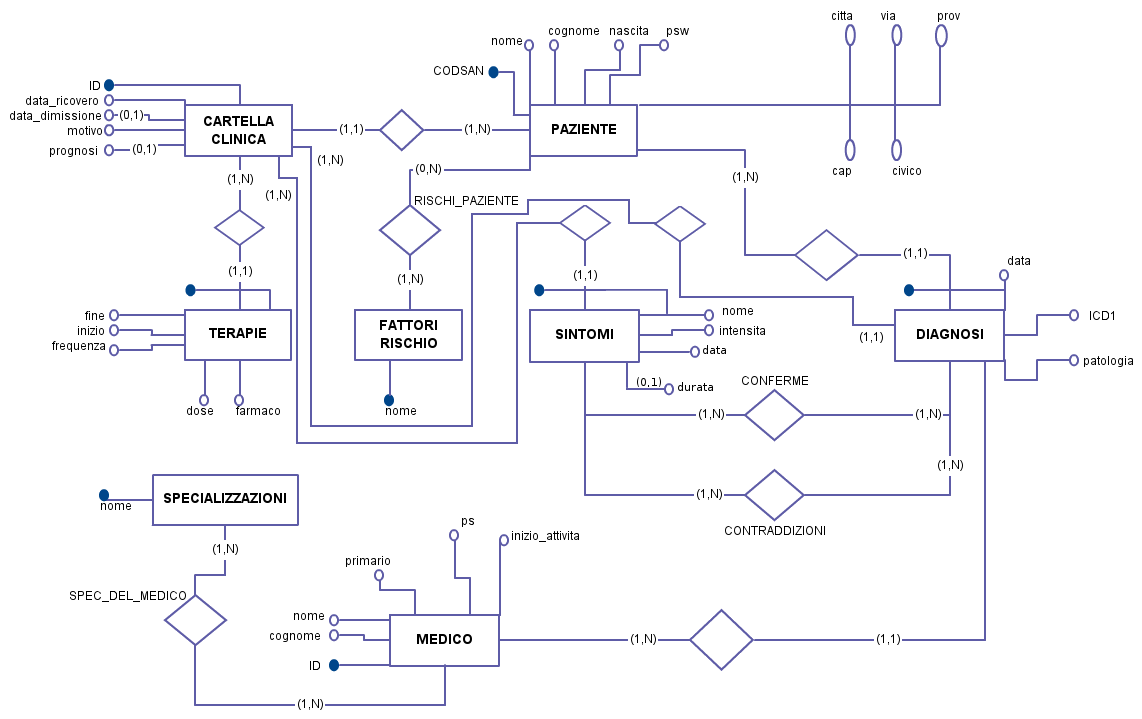
\includegraphics[scale=0.45]{ER.png}
}
 \end{center}
\vfill
\newpage
{\large Elenco delle relazioni:}\newline

\begin{enumerate}

\item Relazione TERAPIE - CARTELLA CLINICA:

\begin{itemize}[leftmargin=0.5cm, topsep=0.25cm, itemsep=0.2cm]

\item Cardinalità (1,1), una TERAPIA è associata univocamente ad una CARTELLA CLINICA
\item Cardinalità (1,N), ad una CARTELLA CLINICA può corrispondere più TERAPIE

\end{itemize}

\item Relazione CARTELLA CLINICA - PAZIENTE:

\begin{itemize}[leftmargin=0.5cm, topsep=0.25cm, itemsep=0.2cm]

\item Cardinalità (1,1), una CARTELLA CLINICA è associata univocamente ad un PAZIENTE
\item Cardinalità (1,N), ad un PAZIENTE può corrispondere più CARTELLE CLINICHE

\end{itemize}

\item Relazione CARTELLA CLINICA - SINTOMI:

\begin{itemize}[leftmargin=0.5cm, topsep=0.25cm, itemsep=0.2cm]

\item Cardinalità (1,N), ad una CARTELLA CLINICA può corrispondere uno o più SINTOMI
\item Cardinalità (1,1), un SINTOMO è associato univocamente ad una CARTELLA CLINICA

\end{itemize}

\item Relazione CARTELLA CLINICA - DIAGNOSI:

\begin{itemize}[leftmargin=0.5cm, topsep=0.25cm, itemsep=0.2cm]

\item Cardinalità (1,N), ad una CARTELLA CLINICA può corrispondere una o più DIAGNOSI
\item Cardinalità (1,1), una DIAGNOSI è associata univocamente ad una CARTELLA CLINICA

\end{itemize}

\item Relazione PAZIENTE - FATTORI RISCHIO:

\begin{itemize}[leftmargin=0.5cm, topsep=0.25cm, itemsep=0.2cm]

\item Cardinalità (0,N), ad un PAZIENTE può corrispondere nessuno o più FATTORI RISCHIO
\item Cardinalità (1,N), ad un FATTORE RISCHIO può corrispondere uno o più PAZIENTI

\end{itemize}

\item Relazione PAZIENTE - DIAGNOSI:

\begin{itemize}[leftmargin=0.5cm, topsep=0.25cm, itemsep=0.2cm]

\item Cardinalità (1,N), ad un PAZIENTE può corrispondere una o più DIAGNOSI
\item Cardinalità (1,1), una DIAGNOSI è associata univocamente ad un PAZIENTE

\end{itemize}

\item Relazione SINTOMI - DIAGNOSI:

\begin{itemize}[leftmargin=0.5cm, topsep=0.25cm, itemsep=0.2cm]

\item Cardinalità (1,N), ad un SINTOMO può corrispondere una o più DIAGNOSI
\item Cardinalità (1,N), ad una DIAGNOSI può corrispondere uno o più SINTOMI

\end{itemize}

\item Relazione DIAGNOSI - MEDICO:

\begin{itemize}[leftmargin=0.5cm, topsep=0.25cm, itemsep=0.2cm]

\item Cardinalità (1,1), una DIAGNOSI è associata univocamente ad un MEDICO
\item Cardinalità (1,N), ad un MEDICO può corrispondere una o più DIAGNOSI

\end{itemize}

\item Relazione MEDICO - SPECIALIZZAZIONI:

\begin{itemize}[leftmargin=0.5cm, topsep=0.25cm, itemsep=0.2cm]

\item Cardinalità (1,N), ad un MEDICO può corrispondere una o più SPECIALIZZAZIONI
\item Cardinalità (1,N), ad una SPECIALIZZAZIONE può corrispondere uno o più MEDICI

\end{itemize}

\end{enumerate}

Per identificare il primario, è stato utilizzato l'attributo ``primario'' dell'entità ``medico'' come stringa contenente ``si'' o ``no'' a seconda che fosse primario o no. 

\newpage

\part{Schema Logico}
 \begin{center}

 \centering
 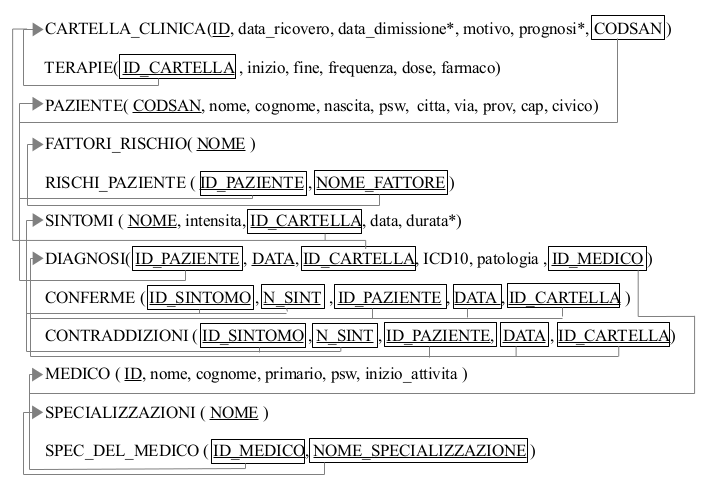
\includegraphics[scale=0.9]{schema_logico.png}

 \end{center}

Questo schema logico rappresenta una visione globale sull'elenco dei vari attributi, sulle chiavi primarie (attributi sottolineati) e sulle relazione tra di essi (i riquadri attorno al nome dell'attributo e la relativa freccia che punta alla relazione).

È stato tradotto nel file ``database.sql'' e popolato tramite il file ``popola.sql''. Quest'ultimo file esegue degli script che contengono molti insert per ogni tabella.
Per generare questi script, sono stati creati dei programmi in grado di generare file .sql con un numero considerevole di insert in base al design del database, in modo da poter testare su grandi numeri il sito (e il comportamento del database).

\newpage
\part{Page Schema}
\begin{lstlisting}
`\textbf{page-schema Homepage unique (}`
	informazioni: link (info, *InfoPage.jsp);
	personale_medico: link (personale, *PersonalePage.jsp);
	patologie: link (patologie, *PatologiePage.jsp);
	login: link (login, *Login.html);
`\textbf{);}`

`\textbf{page-schema InfoPage unique (}`
	primario: String;
	informazioni: text;
	foto: list_of(data[]);
`\textbf{);}`

`\textbf{DB to page-schema InfoPage (}`
	primario: `\color{blue}{select *}` 
		  `\color{blue}{from medico as m}`
		  `\color{blue}{where m.primario = 'si';}`
`\textbf{);}`

`\textbf{page-schema LoginPage unique (}`
	login_paziente: form(
		login: text;
		pw: password;
		invia: submit();
	);
	login_medico: form(
		login: text;
		pw: password;
		invia: submit();
	);
`\textbf{);}`

`\textbf{DB to page-schema LoginPage}`
	`\textbf{parameters(error)}`
	`\textbf{(}`

	login_cliente:
		if(	`\color{blue}{select *}`
			`\color{blue}{from paziente as p}`
			`\color{blue}{where p.codsan = ?codsan?}`
			`\color{blue}{and p.psw = ?psw?}`
		)
		then *PazientePage else *LoginPage
		end;

	login_medico:
		if(	`\color{blue}{select m.*}`
			`\color{blue}{from medico as m}`
			`\color{blue}{where m.id = ?id?}`
			`\color{blue}{and m.psw = ?psw?}`
		)
		then *DiagnosiPage else *LoginPage
		end;
`\textbf{);}`
\end{lstlisting}
\newpage
\begin{lstlisting}
`\textbf{page-schema PazientePage (}`

	dati: (
		codice_sanitario: string;
		nome: string;
		cognome: string;
		data_nascita: string;
		via: string;
		civico: string;
		);

	cartelle_cliniche: list of(
		link(cartella clinica, *CartellaPage);
		);

	fattori_rischio: string;

	elenco_medici: list of(
		nome: string;
		cognome: string;
	);
`\textbf{);}`

`\textbf{DB to page-schema PazientePage}`
	`\textbf{parameters(user)}`
	`\textbf{(}`

	dati: 	`\color{blue}{select p.*}`
		`\color{blue}{from paziente as p}`
		`\color{blue}{where p.codsan = ?codsan?}`
	
	cartelle_cliniche: 
			`\color{blue}{select c.*}`
			`\color{blue}{from cartella\_clinica as c}`
			`\color{blue}{where c.codsan = ?codsan?}`
			`\color{blue}{order by c.id ;}`

	fattori_rischio: 
			`\color{blue}{select r.*}`
			`\color{blue}{from rischi\_paziente as r}`
			`\color{blue}{where r.id\_paziente = ?codsan?}`

	elenco_medici: 	
			`\color{blue}{select distinct m.}`
			`\color{blue}{from paziente as p, medico as m, diagnosi as d}`
			`\color{blue}{where p.codsan = ?codsan?}`
			`\color{blue}{and p.codsan = d.id\_paziente}`
			`\color{blue}{and m.id = d.id\_medico}`
			`\color{blue}{order by m.id ;}`
`\textbf{);}`
\end{lstlisting}
\newpage
\begin{lstlisting}
`\textbf{page-schema CartellaPage (}`
	dati: (
		ID: string;
		dataRic: string;
		motivo: string;
		prognosi: string;
	);
	diagnosi: list of (
		medico: (
			nome_medico: string;
			cognome_medico: string;
		);
		data: date;
		patologia: string;
		icd10: string;
		conferme: list of (
			sintomi: string;
			);
		contraddizioni: list of (
			sintomi: string;
			);
	);
	terapie: list of (
		farmaco: string;
		dose: float;
		posologia: string;
		inizio cura: date;
		fine cura: date;
	);
`\textbf{);}`

`\textbf{DB to page-schema CartellaPage}`
	`\textbf{parameters(cartella)}`
	`\textbf{(}`

	dati:	
		`\color{blue}{select c.*}`
		`\color{blue}{from cartella\_clinica as c, paziente as p}`
		`\color{blue}{where c.id = ?id?}`

	terapie: 
		`\color{blue}{select t.*}`
		`\color{blue}{from terapie as t}`
		`\color{blue}{where t.id\_cartella = ?id?;}`

	diagnosi:
		`\color{blue}{select d.* }`
		`\color{blue}{from diagnosi as d }`
		`\color{blue}{where d.id\_cartella = ?id? }`

	terapie:
		`\color{blue}{select t.*}`
		`\color{blue}{from terapie as t }`
		`\color{blue}{where t.id\_cartella = ?id?}`
`\textbf{);}`
\end{lstlisting}
\newpage
\begin{lstlisting}
`\textbf{page-schema PatologiePage (}`
	patologie: text;
	numero pazienti: int;
`\textbf{);}`

`\textbf{DB to page-schema PatologiePage (}`
	patologie: 	
		`\color{blue}{select d.*}`
		`\color{blue}{from diagnosi as d}`
		
	numero pazienti:
		`\color{blue}{select count(*)}`
		`\color{blue}{from diagnosi}`
		`\color{blue}{where patologia = ?patologia?}` 
		`\color{blue}{and icd10 = ?icd10?}`
		`\color{blue}{group by icd10, patologia}`
		
`\textbf{);}`

`\textbf{page-schema PersonalePage (}`
	primario: text;
	specializzazioni_primario: text;
	
	elenco_medici: list of( medici:text;
				 specializzazioni: text;
				 pazienti_diagnosticati: int;
				 );
`\textbf{);}`

`\textbf{DB to page-schema PersonalePage (}`
	primario: 	
		`\color{blue}{select * }`
		`\color{blue}{from medico as m }`
		`\color{blue}{where m.primario = 'si';}`
		
	specializzazioni_primario: 
		`\color{blue}{select * }`
		`\color{blue}{from spec\_del\_medico as s }`
		`\color{blue}{where s.id\_medico = ?id\_medico? ;}`

	elenco_medici:
		`\color{blue}{select m.* }`
		`\color{blue}{from medico as m }`
		`\color{blue}{order by m.id ;}` 

		`\color{blue}{select * }`
		`\color{blue}{from spec\_del\_medico as s }`
		`\color{blue}{where s.id\_medico = ?id\_medico? ;}`

`\textbf{);}`

`\textbf{page-schema DiagnosiPage (}`
	new_diagnosi: form (
		paziente: string;
		cartella clinica: string;
		data: date;
		ICD10: string;
		sintomi: list of (string);
		tipologia: list of (string);
		durata: list of (int);
	);
`\textbf{);}`

`\textbf{DB to page-schema DiagnosiPage}`
	`\textbf{parameters(error, user, medico)}`
	`\textbf{(}`

	new_diagnosi: `\emph{INSERT INTO DIAGNOSI;}`	
	new_sintomi: `\emph{INSERT INTO SINTOMI;}`
	new_conferme: `\emph{INSERT INTO CONFERME;}`
	new_contraddizioni: `\emph{INSERT INTO CONTRADDIZIONI;}`	
`\textbf{);}`
\end{lstlisting}
\newpage
\part{Struttura dell'applicazione web}

\section{Moduli}
L'applicativo è distribuito secondo lo standard mvc2:

\begin{itemize}[leftmargin=0.5cm, topsep=0.25cm, itemsep=0.2cm]
\item Model: comprende la classe DBMS.java e tutte le classi che descrivono i vari DataBean. DBMS.java si occupa di interrogare il DB e di manipolare i dati al suo interno. La comunicazione con Main.java avviene tramite DataBean in ambo le direzioni. Questa parte è distribuita nelle directory ``bean'' e ``dbms'';
\item Control: comprende la sola classe Main.java, che non è altro che la servlet centrale che si occupa di ricevere tutte le richieste GET e POST, di richiedere a 
DBMS.java tutte le informazioni di cui si ha bisogno, e di inoltrare quest'ultime insieme alla richiesta HTTP alla pagina JSP appropriata.
\item View: comprende tutte le pagine JSP, le librerie javascript usate, le immagini e le foto. Si trova nella cartella ``webapps''.

\end{itemize}

~

Per java ogni interrogazione o manipolazione di dati SQL sono singole transizioni. Se si desidera effettuare una transizione composta da più query è necessario disabilitare l'autocommit ed impostare il livello di isolamento della transizione. Inoltre bisogna gestire esplicitamente il commit e il rollback. Se la transizione accede ad una risorsa non disponibile, allora java lanciera un eccezione ed è compito del programmatore far ricominciare dall'inizio l'intera transizione. Il livello di isolamento più rigido è SERIALIZABLE.

~

Il context tomcat del sito WEB è ``medicina'', mentre il path relativo da context per raggiungere la 
servlet Main è ``home''. La porta per del server è 8080. Quindi l'URL per una richiesta HTTP al 
server sarà del tipo:

~

$http://localhost:8080/medicina/home$

\part{Gestione richieste}

La servlet centrale identifica e gestisce le richieste HTTP sulla base che esse siano GET o POST e 
dipendentemente dal valore del parametro ps passato nella richiesta.
Per le richieste GET, ps può assumere i seguenti valori:

\begin{itemize}[leftmargin=0.5cm, topsep=0.25cm, itemsep=0.2cm]

\item null, si rimanda alla HomePage;

\item info, si rimanda alla pagina di informazioni;

\item login, si rimanda alla pagina di login;

\item cartella, si rimanda alla pagina CartellaPage;

\item patologie, si rimanda alla pagina PatologiePage;

\item personale, si rimanda alla pagina del personale medico (PersonalePage). 

\end{itemize}


Per le richieste di tipo POST (invio valori da un form), ps può assumere i seguenti valori:

\begin{itemize}[leftmargin=0.5cm, topsep=0.25cm, itemsep=0.2cm]

\item paziente, si esegue il login per il paziente;

\item medico, si esegue il login per il medico;

\item diagnosi, si esegue l'insert per la diagnosi.

\end{itemize}

\part{Pagine Web}

Il sito è stato organizzato in maniera servlet-centric, in cui esiste un'unica servlet che gestisce l'apertura delle pagine web in base al parametro ``ps'' presente nella barra url. Per rendere più gradevole l'aspetto del sito, è stato creato un css unico per tutte le pagine del sito.

~

Per gestire il controllo errori, è stata creata una pagina chiamata ``error.jsp'', che viene richiamata in automatico ogni qual volta ci sia un'eccezione nel codice.

~

A differenza delle specifiche, in cui si diceva di inserire nella HomePage le informazioni della divisione ospedaliera (con le foto) e il login, è stato deciso di separare queste due sezioni in rispettive pagine web differenti (Info e Login), in modo da rendere tutto più ordinato, mentre la pagina HomePage funge solo da pagina di menù.

~

Non verranno riportate le query che hanno reso possibile l'acquisizione dei dati da parte del database in quanto sono presenti nel page-schema precedentemente presentato.

~

Infine, tramite una qualsiasi pagina si può raggiungere qualunque altra pagina (che non richieda il login) tramite la barra superiore di selezione (sotto il titolo, di colore viola).

\section{Homepage HTML}

Questa è la pagina principale tramite cui l'utente è in grado di selezionale ogni pagina che vuole consultare. È stata scritta in html in quanto è una pagina statica e non ha necessità di essere modificata tramite i dati del database.

\section{Info JSP}

Questa pagina presenta delle informazioni statiche e delle immagini linkate presenti nella directory \textit{css/images}. L'unica informazione che ha reso necessario l'utilizzo di un'interrogazione al database è stata quella di ottenere il nome del primario. Per questo fatto, è stato necessario sviluppare una pagina di tipo JSP.

~

Passaggio di parametri: nessuno.

\section{Login JSP}

La pagina di Login è statica in quanto presenta sempre gli stessi form in grado di inviare alla servlet i dati per eseguire il login, però deve essere in grado di stampare un messaggio di errore quando il login non è andato a buon fine (quindi deve essere modificabile). Questi dati vengono inviati con metodo post alla servlet, in modo che non vengano visti sulla barra url; la servlet esegue una query per verificare che nome utente e password corrispondano ad almeno un'istanza nel database. Se nome utente e password corrispondono, si viene reindirizzati alla rispettiva pagina (se si esegue il login come paziente si viene reindirizzati a PazientePage, altrimenti a DiagnosiPage), altrimenti viene stampato un messaggio di errore e si viene reindirizzati nuovamente alla pagina di login.

~

Sono presenti quindi due form: uno per il paziente, in cui si inserisce il codice sanitario e la password, e uno per il medico, in cui si inserisce il suo identificatore (codice sanitario) e la password.


~

Passaggio di parametri: 

\begin{lstlisting}[language=java]
	 if (request.getAttribute("error") != null)
 		error = ((Integer)request.getAttribute("error"));
\end{lstlisting}

\section{PazientePage JSP}

La pagina personale del paziente contiene tutti i dati del paziente memorizzati nel database. La parte sinistra della pagina contiene i dati personali, mentre la parte destra contiene i dati relativi ai medici che lo hanno diagnosticato e alle sue cartelle cliniche. Le cartelle cliniche presentate rimandano alla pagina corrispondente che presenta tutti i dati associati alla cartella clinica. Per ottenere le cartelle cliniche del paziente è stata utilizzata una query (vedere page-schema) ordinando il result set per id.


~

Passaggio di parametri: 

\begin{lstlisting}[language=java]
 if (request.getParameter("user") != null)
	 paziente = (String)request.getParameter("user");

\end{lstlisting}


\section{CartellaPage JSP}

Questa pagina contiene tutti i dati importanti di una cartella clinica che possono interessare al paziente. Vengono presentati in ordine: la data ricovero, la data dimissione, il motivo del ricovero, la prognosi (che può non essere presente), l'elenco di terapie somministrate durante il ricovero (farmaco prescritto, dose, posologia e inizio e fine cura) e l'elenco di tutte le diagnosi effettuate dai medici, riportando il nome del medico che l'ha effettuata, la data, la patologia diagnosticata e i sintomi che confermano o contraddicono la patologia.

~

Anche se non era stato specificato, nelle diagnosi sono stati riportati i sintomi che confermano e contraddicono la diagnosi.

~

Passaggio di parametri: 

\begin{lstlisting}[language=java]
	if (request.getParameter("cartella") != null)
		cartella = (String) request.getParameter("cartella");

\end{lstlisting}

\section{PersonalePage JSP}

Questa pagina contiene tutti i dati del personale medico della divisione ospedaliera.

In primo piano viene presentato il primario e le sue specializzazioni (questo è stato ottenuto da una query); successivamente, in una sezione della pagina in verde (camice del chirurgo) sono presentati i medici, con la data di inizio attività, il numero di diagnosi effettuate e l'elenco delle loro specializzazioni. Ogni dato è presentato su riquadro azzurro (camice del medico di reparto). Questi dati sono ottenuti iterando sul result set ottenuto dalla query descritta nel page-schema.

~

Passaggio di parametri: nessuno.


\section{PatologiePage JSP}

In questa pagina vengono presentate tutte le patologie diagnosticate in reparto, riportando il codice ICD10 e il numero di pazienti a cui è stato diagnosticata la patologia considerata. Per ottenere questi dati, è stata eseguita la query descritta nel page-schema; ottenuto il result set, è stato utilizzato un ciclo for per presentare ogni istanza del database proveniente dal risultato della query.

~

Passaggio di parametri: nessuno.


\section{DiagnosiPage JSP Javascript Ajax} 

Questa è la pagina che contiene più codice di programmazione delle altre, poiché sono state aggiunte delle features che permettono al medico di non commettere errori nell'inserimento di una diagnosi e di rendere facile l'utilizzo di questa pagina.

~

Per inserire una diagnosi con i relativi sintomi, è necessario fare almeno 3 insert: uno per la diagnosi, uno per i sintomi diagnosticati e uno o più per indicare se il sintomo conferma o contraddice la diagnosi.

Riguardo alla diagnosi, è necessario sapere il codice sanitario del paziente e della cartella clinica associata.
Per rendere più facile la manipolazione di questi dati, è stato utilizzato un campo del form generale di tipo select tramite cui si può selezionare il paziente; appena si seleziona il paziente, si attiva un sottoprogramma basato su tecnologia Ajax che esegue una query per sapere l'identificatore di tutte le cartelle cliniche associate al paziente e inserire altrettanti option del successivo campo select della form. Questo rende possibile la selezione della cartella clinica senza scriverla a mano (e quindi commettere probabilmente errori).

~

Oltre a questo, è possibile inserire dinamicamente più sintomi per la diagnosi e anche eliminarli qualora ci fossero stati errori di inserimento. Per sviluppare questa utile feature, sono stati utilizzati varie funzioni Javascript che rendessero trasparente la memorizzazione dei dati, l'aggiunzione e l'eliminazione di questi senza creare problemi all'utilizzatore. 

~

Parametri passati: 
\begin{lstlisting}[language=java]
    if (request.getAttribute("error") != null)
    	error = Integer.parseInt((String)request.getAttribute("error"));
    
    if (request.getParameter("user") != null)
	    medico = (String)request.getParameter("user");

    else if (request.getParameter("medico") != null)
	    medico = (String)request.getParameter("medico");
\end{lstlisting}

\part{Strategie progettuali e considerazioni personali}

Per rendere più realistico il database, sono stati aggiunti dei vincoli sugli attributi:

\begin{itemize}[leftmargin=1.5cm, topsep=0.5cm, itemsep=0.2cm]

\item la cartella clinica deve avere una data di ricovero maggiore o uguale della data di nascita del paziente;

\item la cartella clinica deve avere una data di ricovero minore della data di dimissioni;

\item le terapie devono essere fatte in un arco di tempo compreso tra la data di ricovero e dimissione della cartella clinica corrispondente;

\item le terapie devono avere una data di inizio minore o uguale della data di fine;

\item le diagnosi devono essere fatte in un arco di tempo compreso tra la data di ricovero e dimissione della cartella clinica corrispondente.

\end{itemize}

Considerazioni personali e strategie adottate durante lo sviluppo del progetto:

\begin{itemize}[leftmargin=1.5cm, topsep=0.5cm, itemsep=0.2cm]

\item È stato resa la data dimissione (attributo della cartella clinica) come attributo opzionale in quanto si è pensato che possono esserci delle cartelle cliniche di pazienti ancora ricoverati in reparto (nonostante le specifiche non esplicitassero questo fatto);

\item Realizzazione del DB in modo tale da poter ottenere più relazioni possibili con la cartella clinica;
\item Utilizzo del metodo Hibernate durante la realizzazione del progetto in modo tale da poter semplificare le query, tenendo presente che esse restituivano tanti valori nidificati a cui ci si poteva raggiungere tramite superchiavi;
\item Durante la creazione della pagina relativa alle diagnosi (DiagnosiPage) il campo delle cartelle cliniche viene popolato tramite uno script ajax-json-jquery a seconda del paziente selezionato, in modo tale da evitare l'inserimento manuale di una cartella clinica potenzialmente errata;
\item Per la realizzazione generale della pagina web che gestisce l'intero progetto ci siamo sentiti di renderla più gradevole graficalmente inserendo uno stile di impaginazione html in formato css;
\item È stato utilizzato come ambiente di sviluppo Eclipse, in quanto garantiva il controllo degli errori una buona velocità di programmazione.

\end{itemize}


\part{Tecnologie aggiuntive utilizzate}

\section{Hibernate}

Hibernate è un sistema o piattaforma middleware che offre un'interfaccia tra programmatore e database in modo da semplificare e gestire al meglio in maniera trasparente il database da interrogare o aggiornare. Questo sistema, tramite classi Java che rappresentano le entità del database, permette di avere un mapping tra variabili delle classi e attributi delle entità; in questo modo si può avere accesso agli attributi del database lavorando con i metodi get e set sulle variabili interessate.

Il mapping è reso possibile tramite file xml che chiarificano al sistema come mappare sia gli attributi delle entità sia le relazioni con la rispettiva cardinalità.

~

La progettazione si è incentrata sulla corretta scrittura dei file xml e delle relative classi; si è cercato inoltre di esplicitare quali fossero gli identificatori raggruppandoli in sottoclassi(qualora ce ne fossero più di uno), in modo da rendere ancora più chiara la programmazione: ogni classe avrà una dichiarazione sia di attributi sia di identificatori (quindi la creazione di una sottoclasse).

~

Oltre agli attributi e agli identificatori, si è deciso di associare la classe referenziata tramite attributo esterno alla classe interessata; in questo modo si può avere accesso a tutti i campi della classe referenziata applicando i metodi get e set alla sottoclasse, presente quindi nella classe interessata come variabile instanziata.

~

Come esempio pratico, la classe CartellaClinica ha i seguenti attributi:

\begin{lstlisting}[language=java]

	private String id;
	private Paziente paziente;
	private Date dataRicovero;
	private Date dataDimissione;
	private String motivo;
	private String prognosi;
	private Set terapies = new HashSet(0);
	private Set diagnosis = new HashSet(0);
	private Set sintomis = new HashSet(0);

\end{lstlisting}

Come si può notare, la referenza all'entità Paziente (tramite attributo ``codsan'' nel modello relazionale) è resa tramite la dichiarazione della variabile paziente; quindi tramite una singola interrogazione di una specifica cartella clinica si possono sapere anche i campi del rispettivo paziente associato ad essa.

~

Come metodo di verifica della correttezza della progettazione per il sistema Hibernate, è stato utilizzato un plugin di Eclipse chiamato JBoss Tools, che contiene diverse features per Hibernate e permette di verificare la correttezza sia dei file xml sia delle classi Java a partire dalla descrizione del database.

Bisogna notare inoltre che le relazioni molti-a-molti hanno prodotto una referenza tradotta in Java con un HashSet, in modo da poter aver accesso ad ogni valore semplicemente di questo tipo di entità applicando i metodi set e get a questi HashSet. Questo si è rilevato di notevole importanza in quanto, per sapere la quantità di elementi di un certo tipo associati ad una entità, è bastato vedere la grandezza di questi HashSet utilizzando il metodo size, senza quindi fare un'ulteriore query. È stato necessario però forzare il sistema, in alcuni casi, ad avere un comportamento non ``lazy'', quindi impostando a false tale attributo nel file xml, in modo da caricare in memoria anche le istanze referenziate tramite le relazioni e quindi avere libero accesso ad esse. 

\section{Ajax JSON e JQuery}

Poiché si è voluta rendere facile la scelta dei pazienti e delle relative cartelle cliniche nella DiagnosiPage (per rendere sicuro e affidabile un possibile insert da parte del medico nel database), è stato deciso di utilizzare un'insieme di tecnologie che potessero rendere dinamica la scelta da parte del medico. Sono state utilizzate tre tecnogie di sviluppo web chiamate Ajax, JSON e JQuery.

~

Ajax è una tecnica di sviluppo software per la realizzazione di applicazioni web interattive. Consiste nel creare una servlet Java che riceve parametri da parte di una pagina web (nel nostro caso una JSP); questa servlet elabora i dati e li invia alla pagina chiamante, in modo che possa ricevere dinamicamente dati e quindi modificare il suo aspetto o comportamento.

Si è voluta utilizzare questa tecnologia per rendere dinamica la selezione in un campo del form di tipo select; poiché però questi campi devono essere ``popolati'' con dati provenienti dal database, è stato necessario introdurre la tecnologia JQuery e JSON.

JQuery consiste in un insieme di librerie per semplificare la programmazione web, nel nostro caso è stato utilizzato internamente ad Ajax per eseguire una query sul database e mappare in un LinkedHashMap la risposta. Per inviare poi questa risposta alla pagina web, è stato utilizzato JSON, una teconogia che consente lo scambio di dati tra architetture client-server; in questo modo si passa il risultato del calcolo della servlet alla pagina in maniera trasparente senza usare metodi doGet e doPost.

~

Tutto questo è visibile nella servlet ActionServlet e nell'intestazione della pagina DiagnosiPage.

\end{document}


